\section{Question 5}

\subsection{Stochastic spouse presence ($p_s=0.8$) and fertility only when spouse is present.}

\bigskip

\paragraph{Spouse presence.}

To extend the baseline model, we introduce a stochastic spouse presence. We let the state space be $s_t \in \{0,1\}$, which denotes whether a spouse is present, or not. 

\[
s_t =
\begin{cases}
1 & \text{if a spouse is present} \\
0 & \text{otherwise.}
\end{cases}
\]

Spouse presence therefore follows a stochastic process:

\[
s_{t+1} =
\begin{cases}
1 & \text{with probability } p_s = 0.8, \\
0 & \text{with probability } 1-p_s = 0.2.
\end{cases}
\]

We therefore have to extend the household's state vector relative to the baseline model. The new state space becomes

\[
x_t = (s_t,n_t,a_t,k_t),
\]

where $s_t$ captures spouse presence, $n_t$ the number of children, $a_t$ assets, and $k_t$ human capital.

\paragraph{Bellman equation and budget constraint.}

The household's dynamic optimization problem now incorporates stochastic spouse income. The Bellman equation becomes

\[
V_t(s_t,n_t,a_t,k_t)
=
\max_{c_t,h_t}
\left\{
\frac{c_t^{1+\eta}}{1+\eta}
-
\beta(n_t)\frac{h_t^{1+\gamma}}{1+\gamma}
+
\rho \, \mathbb{E}_t
\left[
V_{t+1}(s_{t+1},n_{t+1},a_{t+1},k_{t+1})
\right]
\right\}.
\]

The budget constraint is also modified because the household receives spouse income when $s_t=1$. 
The period budget constraint becomes

\[
a_{t+1} = (1+r)(a_t + (1-\tau_t)(w_t h_t + s_t y_t) - c_t).
\]

Thus, spouse income increases household resources only in periods when a spouse is present.

\paragraph{Fertility restriction.}

In addition to stochastic spouse presence, fertility is restricted so that births can only occur when a spouse is present. As in the baseline model, at most one birth can occur. Let $p_n$ denote the birth probability when the household is eligible.

If $s_t=1$ and $n_t=0$, a birth occurs with probability $p_n$:
\[
\Pr(n_{t+1}=n_t+1 \mid s_t=1,n_t=0)=p_n,
\]
\[
\Pr(n_{t+1}=n_t \mid s_t=1,n_t=0)=1-p_n.
\]

If a child is already present ($n_t\ge1$), fertility remains unchanged. When $s_t=0$, births cannot occur:
\[
\Pr(n_{t+1}=n_t \mid s_t=0)=1.
\]

Thus, stochastic spouse presence reduces the number of periods in which childbirth is feasible compared to the baseline model.
\paragraph{Simulation results and economic interpretation.}

Figure \ref{fig:stoch_spouse_profiles} compares life-cycle profiles in the stochastic spouse model ($p_s=0.8$) and the baseline model ($p_s=1$).

Three mechanisms explain the differences. First, spouse income becomes stochastic, creating income risk. Households respond with slightly higher labour supply as a precaution against periods without spouse income (hours rise from 1.5864 to 1.5928).

Second, when the spouse is present, additional household income raises average consumption relative to the baseline (from 2.4146 to 2.4279).

Third, fertility declines because births are only possible when a spouse is present. Since spouse presence is stochastic, the number of periods in which childbirth can occur is reduced (average fertility falls from 0.3503 to 0.3050).

Overall, the model introduces uncertainty in household income and fertility opportunities, leading to slightly higher labour supply, somewhat higher consumption when spouse income is realized, and lower average fertility. The simulation confirms this: average hours rise from 1.5864 to 1.5928, average consumption increases from 2.4146 to 2.4279, average fertility falls from 0.3503 to 0.3050, and final wealth declines slightly from $-0.9113$ to $-0.9287$, reflecting the income uncertainty from periods without spouse income.
\begin{figure}[H]
\centering
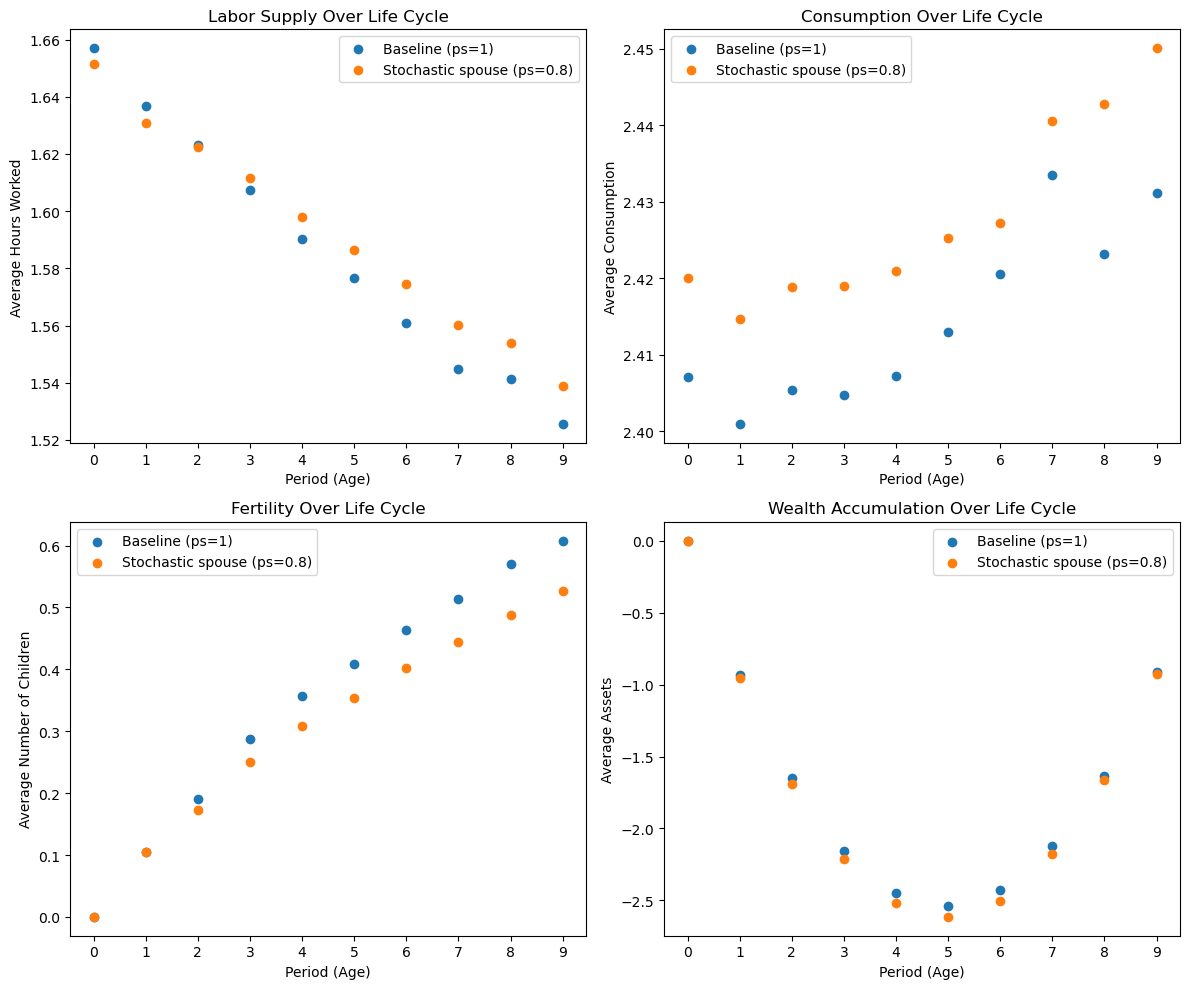
\includegraphics[width=0.5\textwidth]{Billeder/Opgave 5.png}
\caption{Life-cycle profiles: baseline ($p_s=1$) versus stochastic spouse presence ($p_s=0.8$).}
\label{fig:stoch_spouse_profiles}
\end{figure}